In the initial dataset there have been identified a number of inappropriateness which has to be ruled out before working with the data.
These inappropriateness are:
\begin{itemize}
\item Varying dimensions
\item Hugh dimensions
\item Too much noise in the dataset
%\item Positioning
%\item Rotation
\end{itemize}
These problems have been split into two different preprocessing tasks, Dimensional Reduction and Isolation of the whale.

\paragraph{Dimensional reduction}
As mentioned in Section \ref{sec:descr-of-data}, there are varying dimensionality in the dataset. Beside the varying dimensions, is the images too big to process. It is way too time consuming to process machine learning algorithms on images with approximating 3000x2000 pixels in RGB, since the number of dimensions then would be:
\begin{equation}
Dimensions = 3 \times 3000 \times 2000=18.000.000
\end{equation} 
Further is it not given that more dimensions will provide a better result.
Therefore, one preprocessing task is to down scale the images.
The down scale used in this project will be around 45x30 pixels, giving the vectors 4050 dimensions.
Further dimensional reduction is to use gray scale instead of RGB, or simply use binary (\emph{black/white}) generated with a threshold.

\paragraph{Isolating whale}
The problem with reducing the dimensions through scaling, is that the whale is a relatively small part of the images. Figure \ref{fig:scale} shows one of the original images from the dataset and the same image down scaled to 45x30 pixels. As seen from the figure is the whale nearly non existing in the new scale. The whale on the down scaled image is sanding of two pixels.  
Further as the water is noise without information about the whale using computational time on processing it is simply a waste.
\begin{figure}
	\centering
	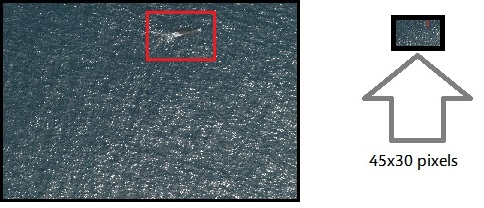
\includegraphics[width=\linewidth]{Images/scale}
	\caption{One picture from the data marked with a red square around the whale, and on the left the same image, down scaled to 45x30 pixels}
\label{fig:scale}
\end{figure}

In order to get more information about the whale it have been decided to develop a system to crop the images to the whale, thereby allowing more information about the actual whale being present in the down scaled images.

\subparagraph{General Principle}
The general principle behind the cropping is  assumption that there is a true difference between what is whale and what is water. Further, do we assume that water pixels, even though there are differences, look more alike than whale pixels and water pixels.
Because of it is assumed that a clustering algorithm could separate water from whale.
In order to lower error rate of this separation there are a number of major parameters:
\begin{itemize}
\item \textit{Smoothing.} By smoothing the image before clustering the pixels, the individual values for the different pixels are equalized based on the neighboring pixels. By doing so, water pixels will look more alike as will individual whale pixels.
\item \textit{Scale.} This will presumably have the same effect as smoothing of the image. But this will also increase performance since it will reduce the number of dimensions.  
\item \textit{Number of clusters.} In order to separate water from whale only two clusters are needed. But this might have some problems if there are more than just water and whale on the image. For instance, does water splash pixels distinguish themselves from both water and whale and by having  only two clusters there would be no control of which cluster these will end up in. They might in fact get one of the clusters for themselves, leaving water and whale in one cluster.
\item \textit{Distance algorithm.} Which algorithm used to determine the distance between pixels might affect of well the separation is done. As mentioned in Section \ref{sec:litterature}, is it suggested to use an euclidean distance
\item \textit{Features.} Using the RGB or gray scale values might not be the best way of separating the data. Another way could be to use redness (how red a pixel is compared to green and blue) since the whale is more red than the water. Further could a value for the distance from average pixel value, for each pixel be used. This might be performing well since most of the image is water therefore the feature would approximately describe one pixels distance from what is water causing all water pixels to be approximately zero and other pixels to be not zero.
\end{itemize}
